\newpage
\section{Realisation}

blah blah blah

\subsection{Erste Schritte}




\textbf{Webserver Verbindungstest}\\
Im oberen Bereich ist der gstreamer Befehl mit dem Audio udpsink host...5000 und Video udpsink...5001. Wireshark detektiert ankommende Pakete im Webserver (ip 85.214.211.169) vom raspberry pi (ip 77.14.37.230) an den UDP Ports 5000 (Audio Paketgröße 451) und UDP 5001 (Video Paketgröße 894).\\

\begin{minipage}{\textwidth}
    \begin{center}
        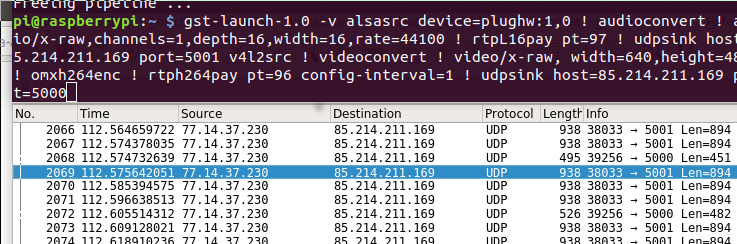
\includegraphics[scale=0.85]{img/wireshark.png} 
    \end{center}
\end{minipage}



